\documentclass{article}
\usepackage[utf8]{inputenc}
\usepackage{graphicx}
\usepackage{subfigure}
\usepackage{booktabs}
\renewcommand{\baselinestretch}{2}

\setlength{\parindent}{0pt}
\begin{document}


\title{\LARGE University of Toronto at Scarborough \\\Large Department of Physical and Environmental Sciences PHYA10\\ \textbf{\huge Vibration Experiment: Studies of Position, Velocity, and Acceleration in Simple Harmonic Motion\\}}
\author{Feiyu Quan \\Partner: Het Pandya \\Partner: Tianao Liu\\Lab Section: PRA 0004\\}
\date{November 25, 2019}

\maketitle

\section{Abstract}
This experiment studies the motion of an object vibrating under the influence of two springs, also known as simple harmonic motion. In this experiment, we analyze the different variables that affect the motion and show their relationship with each other. The variables are position, velocity, and acceleration. We study these relationships by letting the object vibrating between two springs and influenced by their elastic forces. Through this experiment, we can show these relationships by analyzing the graphs of these variables. We believe that the results of this experiment are going to show patterns that are similar to that of the theoretical results of simple harmonic motion.

\section{Introduction}
In this experiment, springs and an object of mass were used to study the kinematics of that object along a straight line. We used the concept of vibrations to analyze the relationships between the variables involved in the motion of objects. The idea of dynamic vibrations allowed us to create the simple harmonic motion of the object with the help of the spring. Simple harmonic motion is the repeated movement of an object back and forth along a plane, where the displacement of the object is equal on both sides of the equilibrium (The Editors of Encyclopaedia Britannica, 2019). The period in which one cycle of that motion is completed is the same for all cycles of that motion (The Editors of Encyclopaedia Britannica, 2019). Vibrations, with the help of constant spring forces, allows us to understand the different variables involved in motion. These variables are position, velocity, and acceleration. This experiment shows the relationship between these variables and how the change in one can have an effect on the other. An experiment was carried out in 2008 in an attempt to show the relationship between force-velocity and determine its effects on resistance training (Schilling, Brian K, et al. 2008). In that experiment, in order to find the relationship between force and velocity, they derived Newton's Second Law (Schilling, Brian K, et al. 2008). It was showed that acceleration is the first derivative of velocity (Schilling, Brian K, et al. 2008). Therefore, in this experiment, we predicted that the variables position, velocity, and acceleration will be related to one another through means of differentiation and integration.

\section{Theory}
We know that simple harmonic motion can be described as a sine or cosine function. Our goal in this part is to derive the equation for the vibration motion in the experiment by starting on some basic assumptions and eventually showing that it matches the patterns of simple harmonic motion.\\
An ideal spring should obey Hooke's law. That is, the force exerted by the spring is proportional to the distance from its equilibrium length:
\begin{figure}[h!]
\centering
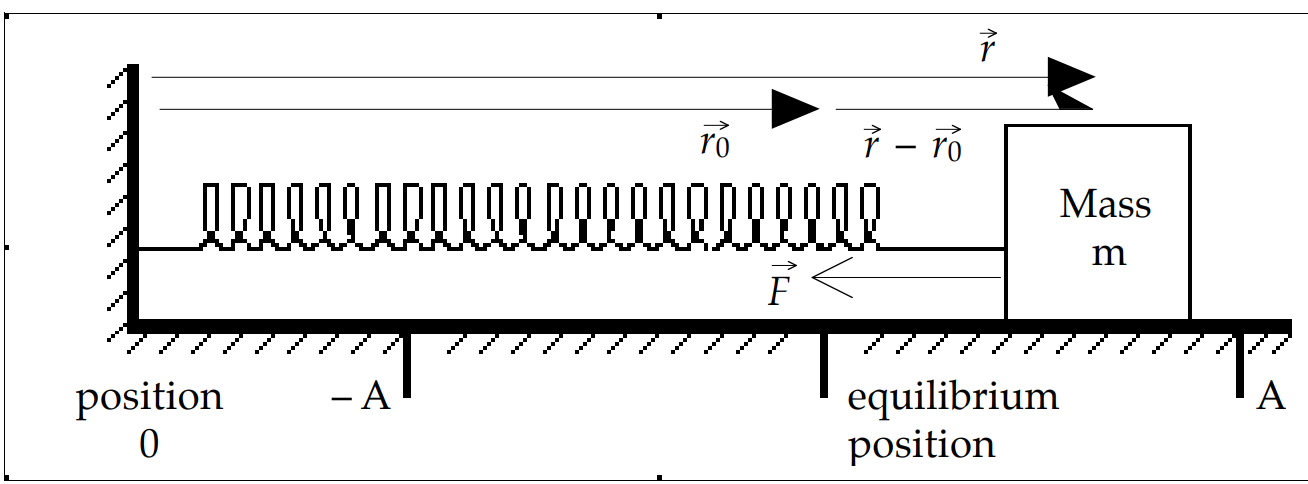
\includegraphics[height=4.2cm]{Figures/figure1.png} 
\caption{\textit{An illustration of an object moving under the influence of a spring.}}
\label{fig:spring and object}
\end{figure}

\begin{equation}
\vec{F}=-k\vec{x}
\end{equation}

where k is the spring constant. There is a negative sign because the force and displacement are in opposite directions.\\
Since there are two springs used in the experiment, we replace \textit{k} with \textit{2k}:

\begin{equation}
\vec{F}=-2k\vec{x}
\end{equation}

Newton’s second law indicates the relationship between force and acceleration:

\begin{equation}
\vec{F}=m\vec{a}
\end{equation}

From equations (2) and (3) we can write that

\begin{equation}
-2k\vec{x}=m\vec{a}
\end{equation}

Since acceleration is the second derivative of displacement, we obtain

\begin{equation}
-2k\vec{x}=m\frac{d^2\vec{x}}{dt^2}
\end{equation}

which is equivalent to:

\begin{equation}
\frac{d^2\vec{x}}{dt^2}+\frac{2k\vec{x}}{m}=0
\end{equation}

Equation (6) is a second-order ordinary differential equation. Solving this equation and assuming that initial position is zero and velocity is in the positive direction, we get

\begin{equation}
x(t)=Asin(t\sqrt{\frac{2k}{m}})
\end{equation}

where \textit{A} is the amplitude of the vibration.\\
This shows that in theory, the vibration in our experiment is indeed described by a sine function and thus the vibration motion should be simple harmonic motion.

\begin{center}
\large\textbf{Experiment Objectives}
\end{center}

In this experiment, we were to analyze the vibrating motion of the system by interpreting phase angles and creating equations of motions that represent the position, velocity, and acceleration of the object. We were also to identify the relationship between these quantities and show how they reflect the functions of listed quantities. 

\section{Experiment Setup}
\begin{center}
\large\textbf{Apparatus}
\end{center}

1.)	Motion Detector: Used to read movements of the object and transmit the collected data to the computer\\2.)	Glider: An object that moves along the air track in order to be analyzed\\3.)	Air Track: Used to create a close to the frictionless surface for the glider to move on\\4.)	Springs: Used to oscillate the glider back-and-forth in an attempt to create simple harmonic motion\\5.) Anchors: Placed a set distance apart in order to fix the movement of glider\\
\begin{figure}[h!]
\centering
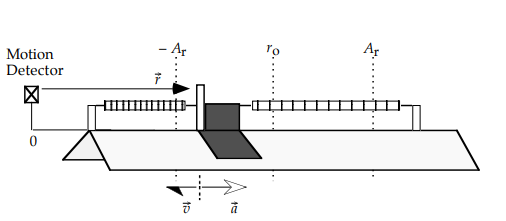
\includegraphics[height=4.2cm]{Figures/figure2.png} \\
\caption{\textit{An image of the experiment setup.}}
\label{fig:air track}
\end{figure}

\begin{center}
\large\textbf{Procedure}
\end{center}

First, we weighed the glider before the air track was set up and was leveled in order to be completely horizontal. The two spring anchors were then set up, the first was placed next to the detector and the second one placed approximately 3 to 4 gliders apart along the ramp. The glider was placed in the middle of the two anchors and the springs were attached on both ends of the glider to each anchor. \\Next, Logger Pro was launched on the computers and a few setting adjustments were made to fit the experiment. The glider was zeroed at the equilibrium point and a test run was run.  We displaced the glider about half a glider length from the equilibrium and released the glider. After one oscillation was completed, we pressed the spacebar on the computer so the computer can start to collect data about the motion of our glider. After the test run, we cleared our data, zeroed the glider at the equilibrium point again, and ran the experiment one more time. This time we got the desired results and saved our data. From here, we created all the graphs and calculated the necessary values that were needed in order to further analyze our experiment.

\section{Results and discussion}
The mass of the glider: $M = 518.1g\pm0.1g$

\begin{table}
\caption{\label{tab:test}\textit{The maximum points for the velocity graph in Figure (3) and the time difference between each point.}}
\begin{tabular}{@{}llllllllll@{}}
\toprule
Point              & 1      & 2      & 3      & 4      & 5      & 6      & 7      & 8      & 9      \\ \midrule
Time(s)            & 0.0323 & 1.62   & 3.39   & 5.10   & 6.815  & 8.56   & 10.3   & 12.0   & 13.7   \\
Velocity(m/s)      & 0.727  & 0.855  & 0.811  & 0.819  & 0.819  & 0.786  & 0.808  & 0.757  & 0.880  \\
Time difference(s) & N/A    & 1.5827 & 1.7750 & 1.7134 & 1.7119 & 1.7447 & 1.7100 & 1.7460 & 1.7120 \\ \bottomrule
\end{tabular}
\end{table}

The mean value for time difference: 1.71196s\\The standard deviation: 0.0572198\\The time difference is the time between every two top points, which can also mean the period of the glider.\\
\begin{figure}[h!]
\centering
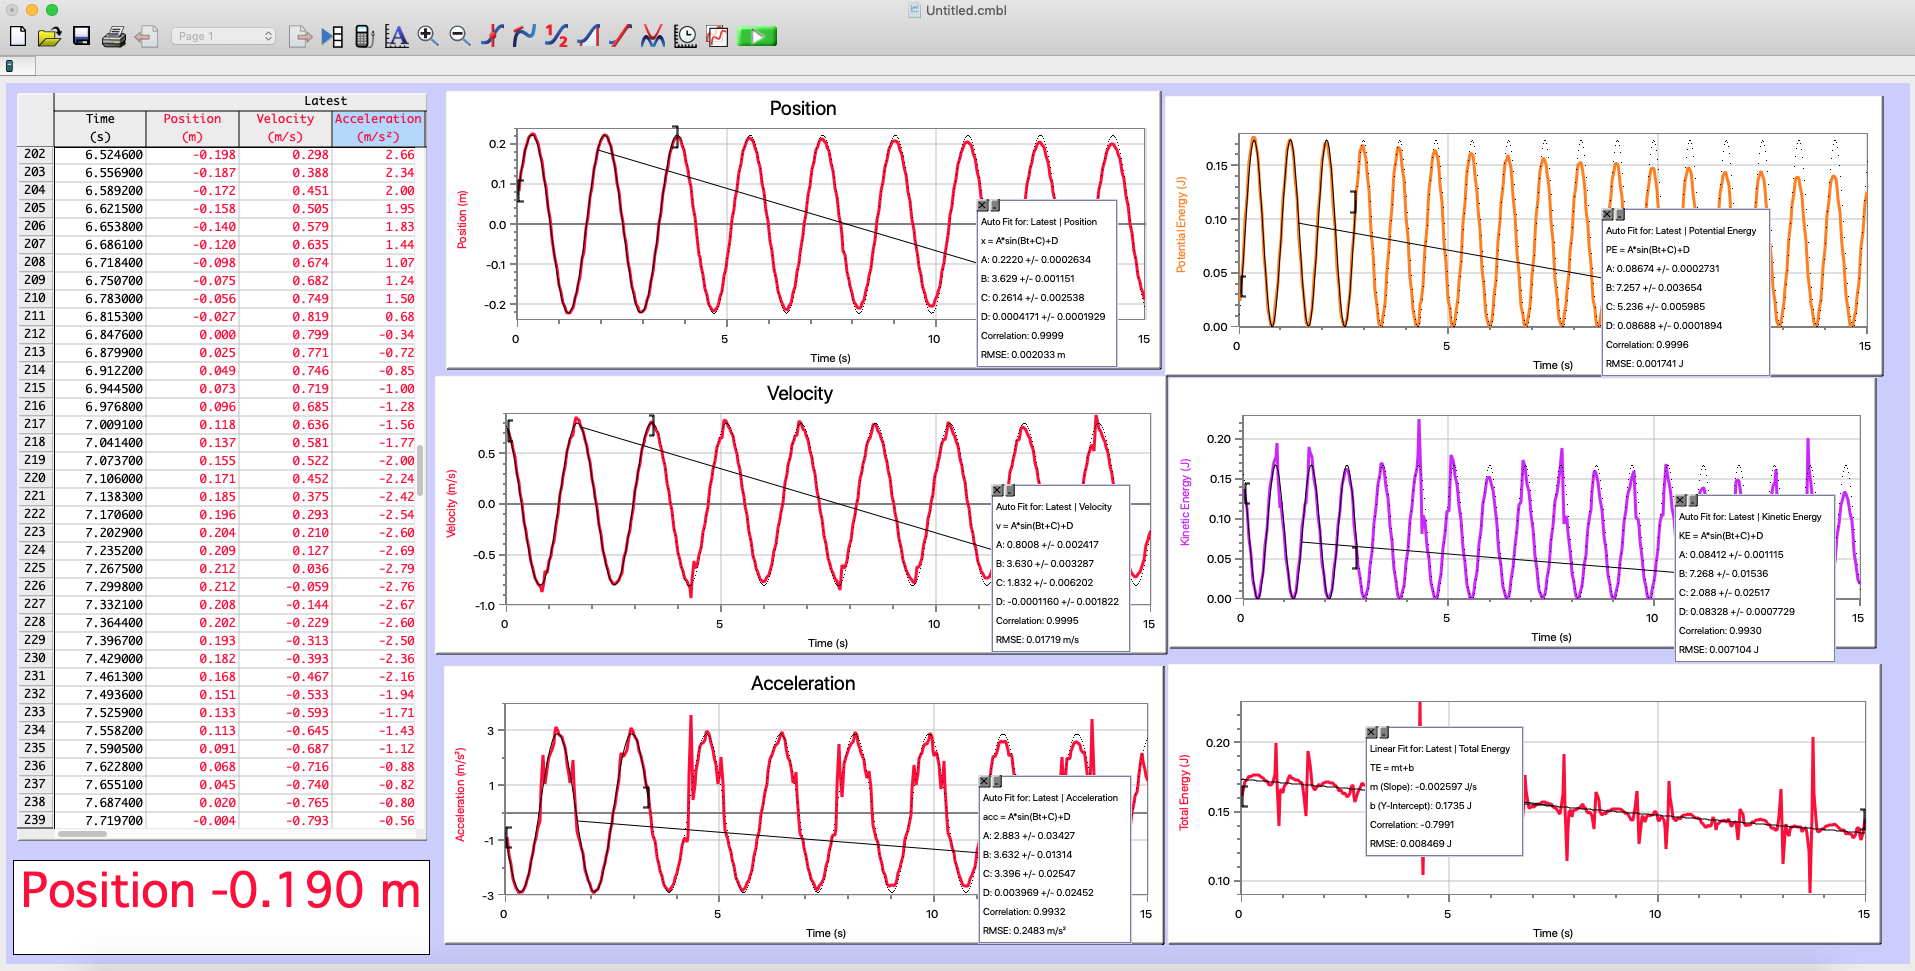
\includegraphics[height=5.4cm]{Figures/figure3.png} \\
\caption{\textit{Graphs describing the motion of the glider and the relationship between different types of energies.}}
\label{fig:Logger Pro graphs}
\end{figure}

From \textit{Table (1)} we can calculate the period (\textit{T}), which is equal to the mean value of time difference in \textit{Table (1)}. Known that the mass of the glider is \textit{M} = 518.1g, we can find the \textit{k} of the spring which is 3.48944. In this experiment, we choose to analyze the position, velocity to find the relationship of energy transfer. For \textit{Figure (3)} we select the first two periods of the glider after we start to collect the data to analyze. The position, velocity, and acceleration graphs are all described by sine functions. We can also see that when potential energy increases, kinetic energy decreases, and vice versa. The equations for position, velocity, and acceleration shown in \textit{Figure (3)} are:

\begin{equation}
x(t)=(0.2220\pm0.0002634)sin((3.629\pm0.001151)t+(0.2614\pm0.002538))+(0.0004171\pm0.0001929)
\end{equation}

\begin{equation}
v(t)=(0.8008\pm0.002417)sin((3.630\pm0.003287)t+(1.832\pm0.006202))+(0.000116\pm0.00001822)
\end{equation}

\begin{equation}
a(t)=(2.883\pm0.03427)sin((3.632\pm0.01314)t+(3.396\pm0.02547))+(0.0003969\pm0.0002452)   
\end{equation}

\begin{center}
\large\textbf{Discussion of Uncertainties and Error Analysis}
\end{center}

The uncertainty for the mass of the glider is $\pm$ 0.1g. From \textit{Table (1)} we use the standard deviation to find the uncertainty of the time period which is  $(0.0572198)/\sqrt{8} = 0.02s$.\\A possible source of error could be that we did not set the spring to be completely horizontal which might result in more work done by the spring force thus decreased energy. From equation (6.) we know that the uncertainty of the mass of the glider and the period might cause the change of \textit{k} of the spring thus affect the final results.\\A possible way of improving the experiment could be lubricating the air track before placing a glider on it, as this will help further decrease the friction force between the glider and the track.

\section{Conclusion}

\begin{center}
\large\textbf{Answers to Lab Manual Questions}
\end{center}

\textbf{Question 1: Are the kinetic and potential energy graphs sinusoidal? Why?}\\
\textbf{Answer:}Yes. From \textit{Figure (3)}, we can see that both the graphs are sinusoidal. We know that

\begin{equation}
K(v)=\frac{mv^2}{2}
\end{equation}

and

\begin{equation}
U(x)=\frac{kx^2}{2}
\end{equation}

Since both velocity \textit{v} and position \textit{x} have sinusoidal graphs, kinetic and potential energy graphs are also sinusoidal.

\textbf{Question 2: What is the maximum kinetic energy (in J)?}\\
\textbf{Answer:} From \textit{Figure (3)}, we can find that the maximum of kinetic energy at the area we analyze in the graph is about 0.195 J.

\textbf{Question 3: What is the maximum potential energy (in J)?}\\
\textbf{Answer:} From \textit{Figure (3)}, we can find that the maximum of potential energy at the area we analyze in the graph is about 0.175 J.

\textbf{Question 4: Is the total energy of your oscillator constant? Why?}\\
\textbf{Answer:} The total energy is not constant. The reason is that although in this experiment we use air track to simulate the frictionless situation, it could not be perfectly frictionless and there is always a part of mechanical energy converted into thermal energy due to friction, resulting in the loss of total energy.

\textbf{Question 5: Why is the frequency of the kinetic energy graph double that of the velocity (or position) graph?}\\
\textbf{Answer:} In one period of the velocity graph, there are 2 points where velocity reaches its extreme value. However, in one period of the kinetic energy graph, there is only 1 point where it reaches its maximum value. By equation (11.) we know that kinetic energy reaches its maximum value only when velocity reaches its extreme value, which means in one period of velocity graph the kinetic energy graph should undergo two periods. We know that:

\begin{equation}
f=\frac{1}{T}
\end{equation}

Thus, this is equivalent to that the frequency of the kinetic energy graph doubles that of the velocity graph.

\textbf{Question 6: Why is the frequency of the potential energy graph double that of the position (or velocity) graph? Explain this doubling in physical and mathematical terms.}\\
\textbf{Answer:} In one period of the position graph, there are 2 points where the position reaches its extreme value. However, in one period of the potential energy graph, there is only 1 point where it reaches its maximum value. By equation (12.) we know that potential energy reaches its maximum value only when the position reaches its extreme value, which means in one period of velocity graph the kinetic energy graph should undergo two periods. By equation (13.) we know that this is equivalent to that the frequency of the position energy graph doubles that of the position graph.

\textbf{Question 7: Devise another question about energy and then answer it.}\\
\textbf{Devised Question: Why does potential energy reach its maximum value when kinetic energy reaches its minimum value and vice versa?} \\
\textbf{Answer:} The total energy is the sum of potential energy and kinetic energy. When either potential or kinetic energy reaches its maximum value, it equals to exactly the value of total energy, which means there could not be any other form of energy left.

\textbf{Question 8: What does it mean to say there is energy “lost”? You should be able to calculate this energy loss in Joules per second by fitting a function (what function?) to the graph. Figure 4-10 provides a clue.}\\
\textbf{Answer:} Since the experiment is not conducted under perfectly frictionless circumstances, the mechanical energy, i.e. the total energy is not conserved and part of it is converted into thermal energy. 

\begin{figure}[h!]
\centering
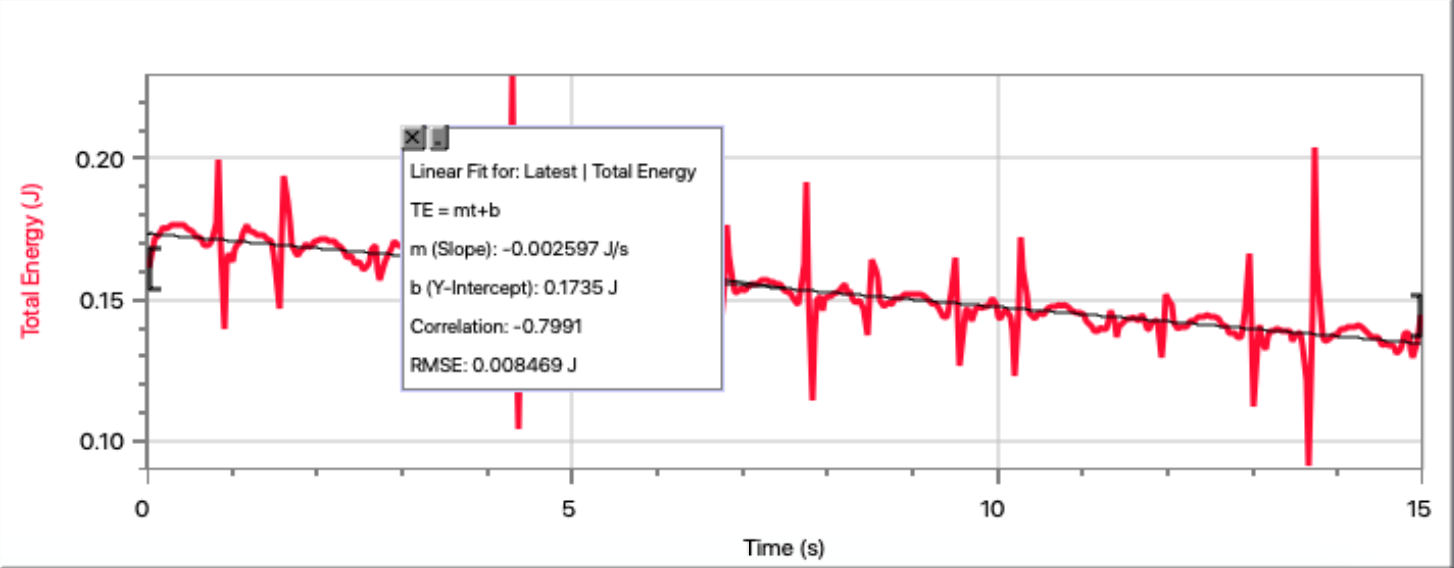
\includegraphics[height=4.5cm]{Figures/figure4.png} \\
\caption{\textit{Graph of the total energy (mechanical energy).}}
\label{fig:Logger Pro graph}
\end{figure}

From \textit{Figure (4)}, we can see that the graph is oscillating while slowing declining. The rate of loss of energy is exactly the slope of the graph, which is 0.002597 J/s.

\textbf{Question 8: Where is this energy going? Can it be retrieved?}\\
\textbf{Answer:} The lost energy is converted into thermal energy and can not be retrieved. 

\begin{center}
\large\textbf{Final Conclusion}
\end{center}

From our fitting of the graph, we can see that position, velocity, and acceleration vs. time graphs all follow the pattern of the sine function. This indicates that the vibration motion in our experiment is simple harmonic motion as predicted in the theory part. 

\LARGE\textbf{References}

\normalsize The Editors of Encyclopaedia Britannica. “Simple Harmonic Motion.” \textit{Encyclopædia Britannica,} Encyclopædia Britannica, Inc., 5 Apr. 2019, https://www.\\britannica.com/science/simple-harmonic-motion.

Schilling, Brian K et al. “Force-velocity, impulse-momentum relationships: implications for efficacy of purposefully slow resistance training.” \textit{Journal of sports science and medicine} vol. 7,2 299-304. 1 Jun. 2008

Wikipedia contributors. "Spring (device)." \textit{Wikipedia, The Free Encyclopedia.} Wikipedia, The Free Encyclopedia, 25 Sep. 2019. Web. 24 Nov. 2019.

\end{document}
